\documentclass[english]{article}
\title{Model for iTasks agents}
\author{Wessel van Staal}
\usepackage{hyperref}
\usepackage[parfill]{parskip}
\usepackage[english]{babel}
\usepackage{amsmath}
\usepackage{amsfonts}
\usepackage{amssymb}
\usepackage{apacite}
\usepackage{graphicx}
\usepackage{caption}
\usepackage{subfigure}
\usepackage{listings}
\usepackage{enumerate}
\usepackage{syntax}
\usepackage{alltt}
\graphicspath{{/latex_objects/}}
\usepackage{tikz}
\usepackage{qtree}
\usetikzlibrary{positioning, shapes, arrows, decorations.pathreplacing}

\usepackage{listings}
\usepackage{lstautogobble}

\newcommand{\nat}{\mathbb{N}}
\newcommand{\pow}{\mathcal P}

\lstset{basicstyle=\ttfamily,
  mathescape=true,
  tabsize=2,
  autogobble}
  
\begin{document}
\maketitle

\section{Idea}

In this document, we present an idea for an agent model for iTasks. We give an informal explanation of the features. Each agent is associated with an unique name and is defined in terms of beliefs and activities to complete tasks. Beliefs are assertions about the environment perceived to be true by the agent. An example of a belief is '$direction := "North"$' where an agent believes its current direction is to the north. An agent can use these beliefs to make decisions when performing tasks. 

Activities are descriptions of actions the agent can perform to complete tasks, given that the tasks are available and preconditions are met. Each activity is a combination of a \textit{pattern} on the tasks at hand and a possible guard condition. An example of a pattern is a match on a tasks with a particular identifier. An activity can be used once the pattern match succeeds and the guard condition holds. Each activity concludes with a sequence of actions to be performed on tasks and beliefs that are updated. 

Important is that agents only produce the input necessary to complete tasks, but do not define tasks themselves. The task specification is defined in a separate iTasks model. They do reason about how to complete a task.

Agents obtain information about the environment by inspecting their beliefs and querying the value of tasks. The idea is that agents obtain their information from iTasks in the same way humans do: through observing the information that tasks present. 

\section{Overview}

\begin{figure}[h!]
  
 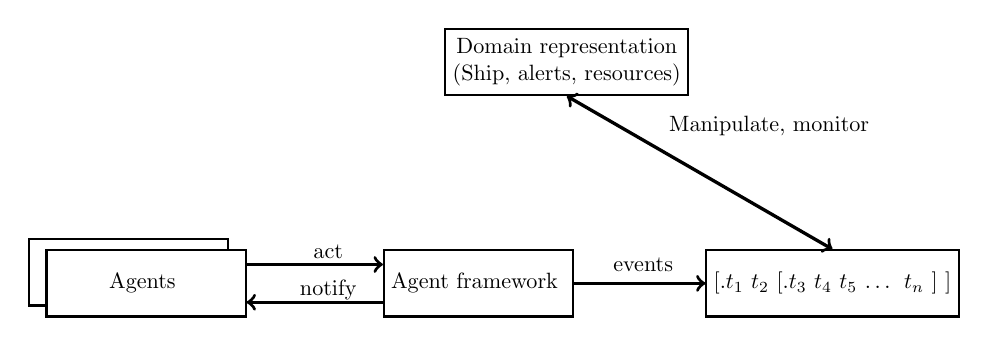
\begin{tikzpicture}[thick,scale=0.8, every node/.style={transform shape}]


\node[rectangle, draw, align=center, xshift=25em, yshift=10em, rotate=0, minimum height=3em](domain){Domain representation \\ (Ship, alerts, resources)};

\node[rectangle, draw, align=center, xshift=5.2em, yshift=0.5em, rotate=0, minimum height=3em, minimum width=9em](agents){ 
};

\node[rectangle, draw, align=center,fill=white, xshift=6em, yshift=0em, rotate=0, minimum height=3em, minimum width=3em, minimum width=9em](agents){ Agents
};

\node[rectangle, draw, align=center,fill=white, xshift=21em, yshift=0em, rotate=0, minimum height=3em, ](framework){ Agent framework
};



\node[rectangle, draw, align=center, xshift=37em, yshift=0em, rotate=0, minimum height=3em](tasks){\Tree [.$t_1$ $t_2$ [.$t_3$ $t_4$ $t_5$ {\ldots} $t_n$ ] ]};


\draw[<->, very thick] (domain.south) to (tasks.north);
\node at (12,2.5) (refine) {Manipulate, monitor};


\draw[<-, very thick] ([yshift=0.3 cm]framework.west) to ([yshift=0.3 cm]agents.east);
\node at (5,0.5) (refinde) {act};
\draw[->, very thick] ([yshift=-0.3 cm]framework.west) to ([yshift=-0.3 cm]agents.east);
\node at (5,-0.1) (refinde) {notify};

\draw[->, very thick] ([]framework.east) to (tasks.west);
\node at (10,0.3) (refinde) {events};

\end{tikzpicture}

\end{figure}

In order to implement the idea as proposed, we need to consider how agents are implemented and how they communicate with iTasks. We have the following requirements:

\begin{itemize}
\item Agents should be able to inspect values of tasks.
\item Agents must be able to work on tasks by giving input to editors or taking actions.
\item Agents must be able to make decisions about how to complete tasks.
\item Agents must be notified when a value of their active tasks changes or when a new task is assigned to them.
\end{itemize}

We define the architecture as follows. Agents communicate with iTasks through a framework that translates output from agents to events that are interpreted by the iTasks server. Further, the framework takes care of executing the agents when the iTasks server reports changes in the task model (e.g. a new task is assigned to an agent). The idea is that communication is done by exchanging JSON messages with the HTTP protocol. This way, we can reuse the existing iTasks web service architecture.

We require at least following changes to iTasks:

\begin{itemize}
\item Agents need to be able to identify tasks: we need to be able to 'tag' tasks with some identifier. This can be implemented by adding a extra combinator to the iTasks DSL. 
\end{itemize}

\section{Representation in Clean}

We model agents as transition relations in Clean: 

\begin{lstlisting}

:: AgentActivity :: s [AgentTask] -> Maybe (s, [AgentAction])

:: Agent s = 
   { id        :: String
   , activity  :: AgentActivity s
   }
\end{lstlisting}

The idea is that beliefs and other internal state is encapsulated in some type $s$, which can be different for each individual agent. Based on this state and tasks that are currently active, the agent can decide what actions to perform on what tasks. We represent this with the \textit{AgentActivity} type.

We need to consider that each task can have a value of some different type. Agents need to be able to make decisions based on these values. We adopt the method that iTasks uses: values are stored internally as JSON representations. The $tag$ field represents tag annotations in the iTasks program such that the agent is able to identify tasks. This is feature is yet to be implemented in iTasks. This representation is not yet complete, it is likely that more information is required.

\begin{lstlisting}
:: AgentTask = 
   { taskId :: TaskId
   , tag    :: String
   , value  :: JSONNode
   }
\end{lstlisting}

We represent actions performed by agents as follows, where we only distinguish between \textit{edit} and \textit{act} actions. Edit actions mutate editors in iTasks to update values. Act actions execute actions defined in step combinators.

\begin{lstlisting}
:: AgentAction = EditAction TaskId JSONNode
               | ActAction  TaskId String
\end{lstlisting}

We want to be able to specify when it is appropriate to execute actions to complete a task. In order to do this in a concise manner, we introduce a pattern type. A pattern takes a list of active tasks and the current agent state and yields some value if the pattern succeeds. We currently only have the $task$ primitive to match on tasks with a certain tag, but this can be expanded in the future. Patterns can be composed with the usual bind operator and the $-\&\&-$ and $-||-$ operators. 

\begin{lstlisting}
:: Pattern a s :== s [AgentTask] -> Maybe a

return :: a -> Pattern a s
(>>=)  infixl 3 :: (Pattern a s) (a -> Pattern b s) -> Pattern b s
(-&&-) infixr 5 :: (Pattern a s) (Pattern b s) -> Pattern (a, b) s
(-||-) infixr 4 :: (Pattern a s) (Pattern a s) -> Pattern a s
(-|-)  infixr 3 :: (Pattern a s) (a s -> Bool) -> Pattern a s

task :: String -> Pattern AgentTask s
\end{lstlisting}

If a pattern holds, we would like to update the internal state of the agent and produce a list of actions to execute. We do this with the $==>$ operator. Activities can be composed with $\textless |\textgreater$. This composition works as follows: if the first activity succeeds, the second activity is disregarded. Otherwise, the second activity is attempted.

\begin{lstlisting}
(==>) infixr 2 :: (Pattern a s) (a s -> [AgentAction]) -> AgentActivity s

(<|>) infixr 1 :: (AgentActivity s) (AgentActivity s) -> AgentActivity s
\end{lstlisting} 

We define a few helper functions to define actions and to obtain values from tasks:

\begin{lstlisting}
value :: AgentTask -> a | JSONDecode{|*|} a

edit :: AgentTask a -> AgentAction | JSONEncode{|*|} a

act :: AgentTask -> AgentAction
\end{lstlisting}

\section{Examples}

This example shows agents suitable for the 'planning dates' example in Bas Lijnse's thesis, where we assume that the interactive tasks are labelled. The goal of participants is to select a date for a meeting. The coordinator proposes a few initial dates and other participants select one date. The coordinator makes the final decision.

\begin{lstlisting}
:: CoordinatorState = { favoriteDate :: Date }

coordinator :: Agent CoordinatorState
coordinator = { id = "Coordinator", activity = coordinatorActivity }

coordinatorActivity :: AgentActivity CoordinatorState
coordinatorActivity = enterInitialDates <|> makeDecision	  
where
	enterInitialDates = 
		task "enterDates"
		-&&-
		task "enterDatesContinue"
		==> (\(enterDates, continueButton) s. 
			(s, [
			  	 edit enterDates initialDates
			    ,act continueButton
			  	]))
	makeDecision = 
			task "makeDecision"
			-&&-
			task "monitorDateTimes"
			-|- (\(_, monitor) s. any ((==)s.favoriteDate) (value monitor))
			==> \(decide, _) s. (s, [act decide])
	initialDates = [{Date|day=1, mon=1, year=2013},
			{Date|day=2, mon=1, year=2013}]
			  
chooser1 :: Agent Void
chooser1 = 
	{ id = "DateChooser1", 
		activity = dateChooserActivity {Date|day=1, mon=1, year=2013} }

chooser2 :: Agent Void
chooser2 = 
	{ id = "DateChooser1", 
		activity = dateChooserActivity {Date|day=2, mon=1, year=2013} }

dateChooserActivity :: Date -> AgentActivity Void
dateChooserActivity dt = task "chooseDate"
				 		-&&-
				 		task "chooseDateDone"
				 		==> \(chooseDate,done) s. (s, [edit chooseDate dt, act done])
\end{lstlisting}

\begin{lstlisting}
dateChooser :: Date -> AgentActivity Void
dateChooser dt = task "chooseDate" -&&- task "chooseDateDone"
							   ==> \(chooseDate,done) s.
							  				(s, [edit chooseDate dt, act done])
\end{lstlisting}
\end{document}